\chapter{Control Architecture}
\section{Simple Inverted Pendulum Mode}
The simple inverted pendulum is the most basic model used to simplify humanoids' body. The basis of the pendulum are a mass $m$ linked to a pivot point $0$ by means of a massless link of longitude $l$ as in Figure \ref{fig:pendulo_inv}.

The mass $m$ represents the total mass of the modelled system, a humanoid robot in this case, located at its Centre of Mass (CoM), and the longitude $l$ is the distance between the pivot point to the CoM. Its dynamical model in a planar, for example XZ case, is expressed by the equation \ref{eq:pendulo}, if gravitational force is considered the only force acting in the system.

\begin{figure}
\centering
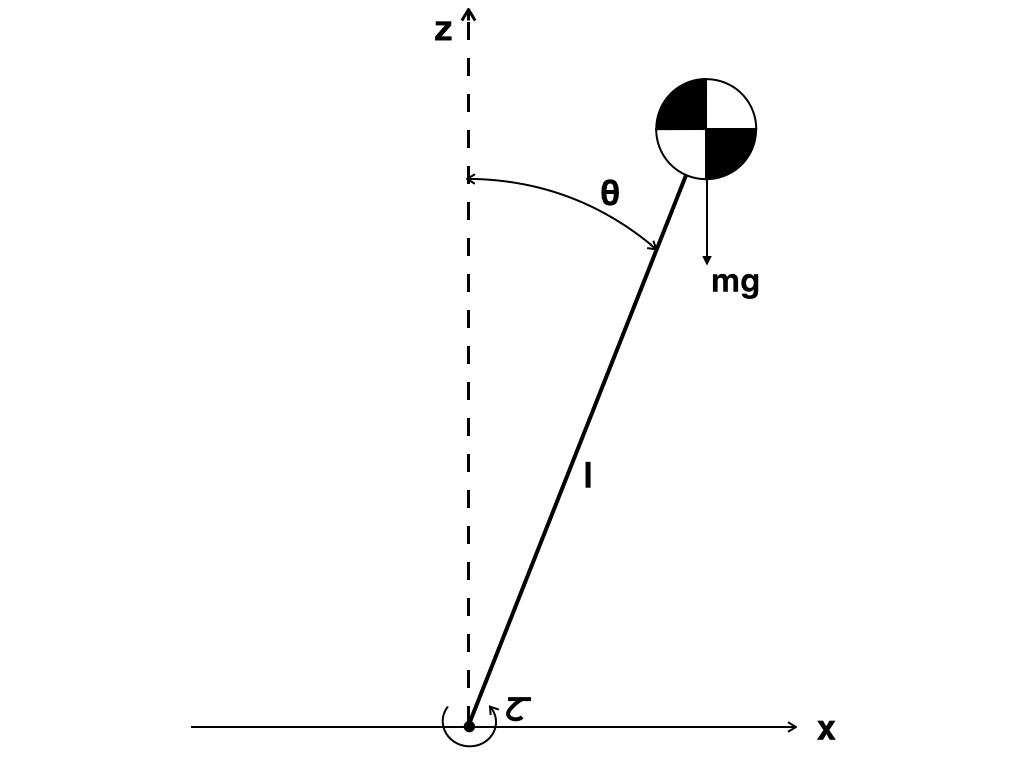
\includegraphics[scale=0.25]{pendulo_inv.png}
\caption{Single inverted pendulum.}
\label{fig:pendulo_inv}
\end{figure}

\begin{equation}
\tau_0 = ml^2 \ddot{\theta} - mgl\sin\theta
\label{eq:pendulo}
\end{equation}

where $\tau_0$ is the torque generated by the ankle joint, $\theta$ its angular position and $l$, the distance between the joint and the CoM. It is assumed that angles are small enough and $\sin\theta = 1$. Then, equation \ref{eq:pendulo} changes to equation \ref{eq:pendulo2}
\begin{equation}
\tau_0 = ml^2 \ddot{\theta} - mgl\theta
\label{eq:pendulo2}
\end{equation}

The main complexity of this model is the fact that equation \ref{eq:pendulo2} does not give the possibility of controlling the ZMP by angular position of the ankle joint. To overcome this problem, the inverted pendulum model can be slightly modified. The link of the pendulum which connects the ankle joint to the concentrated mass (CoM) is generally assumed to be rigid. However, in the real humanoid mechanism it is flexible because the leg length is relatively long and the mechanical structure suffers form flexibility and small backlashes. Because of this compliance, the humanoid robot exhibits the characteristics of a lightly damped structure \cite{Kim2004}. For example, in a static case when the ankle joint is under position control, a pushing external force can easily excite an oscillation. This oscillation exists even when the position error in every joint is zero. This phenomenon is prevalent in the fast dynamical gait; therefore it is very imortant to implement a control mechanism allowing ZMP fast correction considering the stiffness of the humanoid robot links. The most suitable model in this case will be a single mass inverted pendulum with compliant joint as shown in Figure \ref{fig:pendulo_elast}, where $u$ denotes the ankle joint reference angle and $\theta$ denotes the actual inclined angle produced by the compliance of the mechanical structure of the humanoid, $k$ denotes the stiffness of the leg and $\tau_0$ is the torque produced by the motor of the ankle joint to place the inverted pendulum into the desired angular position. Then, the torque $\tau_0$ should be expressed as:

\begin{equation}
\tau_0 = k(\theta - u)
\label{eq:pendulo3}
\end{equation}

\begin{figure}
\centering
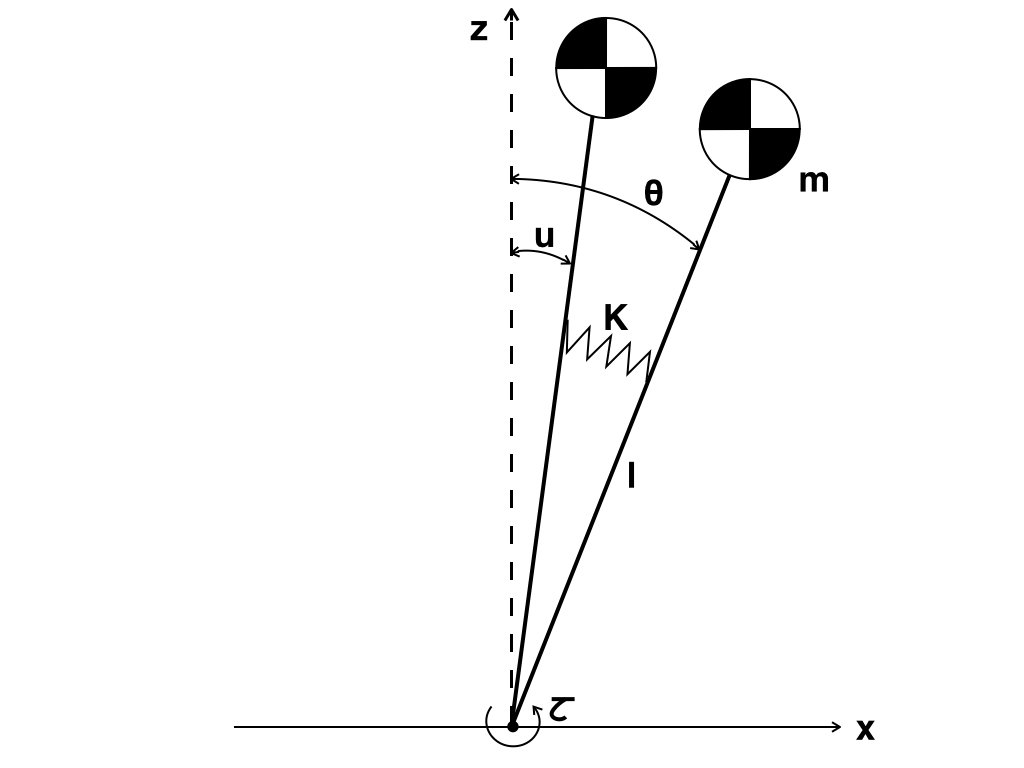
\includegraphics[scale=0.25]{pendulo_elast.png}
\caption{Single inverted pendulum with compliant joint.}
\label{fig:pendulo_elast}
\end{figure}

Taking the Laplace transform of equation \ref{eq:pendulo2}, it is obtained: 
\begin{equation}
T(s) = mgl\theta(s)- ml^2s^2\theta(s) 
\label{eq:par}
\end{equation}

The Laplace transform of equation \ref{eq:pendulo3} is:
\begin{equation}
T(s) = k(\theta(s) - U(s))
\label{eq:par2}
\end{equation}

Reflecting $\theta(s)$ from equation \ref{eq:par2} and placing it into the equation \ref{eq:par} and simplifying, the transfer function is obtained:
\begin{equation}
\frac{T(s)}{U(s)} = k \frac{-s^2+(\beta - \alpha)}{s^2 + \alpha}
\label{eq:TFpar}
\end{equation}

where:
\begin{equation}
\alpha = \frac{k-mgl}{ml^2}
\end{equation}
\begin{equation}
\beta = \frac{k}{ml^2}
\end{equation}

On the other hand, from equation \textcolor{red}{[REF ECUACION zmp]} relating the moment produced by the ground reaction force around $y$ axis with $x$ ZMP direction (the planar XZ case of the inverted pendulum is considered) we can get:
\begin{equation}
\tau_y = -mgx_{ZMP} = - F_z x_{ZMP}
\label{eq:zmp}
\end{equation} 

and then the Laplace transform of the equation \ref{eq:zmp} is:
\begin{equation}
\tau_y(s) = - F_z x_{ZMP}(s)
\label{eq:TFzmp}
\end{equation}

For the static equilibrium of the system, the moment generated y the motor of the ankle join should compensate the moment produced by the ground reaction force:
\begin{equation}
\tau_0 = \tau_y
\end{equation}

The relation between $\tau_y$ and $x_{ZMP}$ is lineal, therefore, placing \ref{eq:TFzmp} into \ref{eq:TFpar} we get the following transfer function relating ZMP to ankle joint position: 
\begin{equation}
\frac{x_{ZMP}(s)}{U(s)} = - k_1 \frac{-s^2+(\beta - \alpha)}{s^2 + \alpha}
\end{equation}

where $k_1 = \frac{k}{mg}$.

In the equation \ref{eq:TFpar} $x_{ZMP}(s)$ is the output and $U(s)$ is the input of the system. It allows for the ZMP of the humanoid robot to be contolled by the position of its ankle joint. From transfer function equation, we can obtain the space state model equations:
\begin{equation}
\begin{bmatrix}
\dot{x_1} \\
\dot{x_2}
\end{bmatrix} 
= 
\begin{bmatrix}
0 & 1 \\
-\alpha & 0
\end{bmatrix}
\begin{bmatrix}
x_1 \\
x_2
\end{bmatrix}
+
\begin{bmatrix}
0 \\
1
\end{bmatrix}
u
\label{eq:state_space}
\end{equation}
\begin{equation}
y = \begin{bmatrix}
-k_1\beta & 0 
\end{bmatrix}
+ \begin{bmatrix}
k_1
\end{bmatrix}
u
\label{eq:state_space_out}
\end{equation}

where $ x_1 $ and $ x_2 $ are state variables and $y$ is the output of the system, then the $x_{ZMP}$


\section{Feedback in state space. The Linear Quadratic Regulator}

The quadratic optimal control method is one of the control methods applied in state space systems and it provides a systematic way of computing the state feedback control gain matrix \cite{Ogata}.
Given the state space system equation
\begin{equation}
\dot{x} = Ax+Bu ,
\label{eq:sseq}
\end{equation}
the LQR determines the matrix $K$ of the optima control vector
\begin{equation}
u(t) = -Kx(t)
\label{eq:control}
\end{equation}
so as to minimize the performance index
\begin{equation}
J = \int_{0}^{\infty}(x^{T}Qx+u^{T}Ru) dt
\end{equation}

where $Q$ is a positive-definite (or positive-semidefinite) Hermitian or real symmetric matrix and $R$ is a positive-definite Hermitian or real symmetric matrix. Note that the matrices $Q$ and $R$ determine the relative importance of the error and the expenditure of the energy of the control signals.
The linear control law given by equation \ref{eq:control} is the optimal control law. Therefore, if the unknown elements of the matrix $K = [K_1 \quad K_2]$ are determined so as to minimize the performance index, then $u(t) = -Kx$  is optimal for any initial state $x(0)$. The block diagram showing the optimal configuration for the single inverted pendulum system is presented in Figure \ref{fig:block_diagram}. The controller maintain desired ($x_{ZMP}$) position of the single pendulum close to zero. Thus, the reference input of the control system in Figure [REF] is not zero.?????
\begin{figure}[!hbt]
\centering
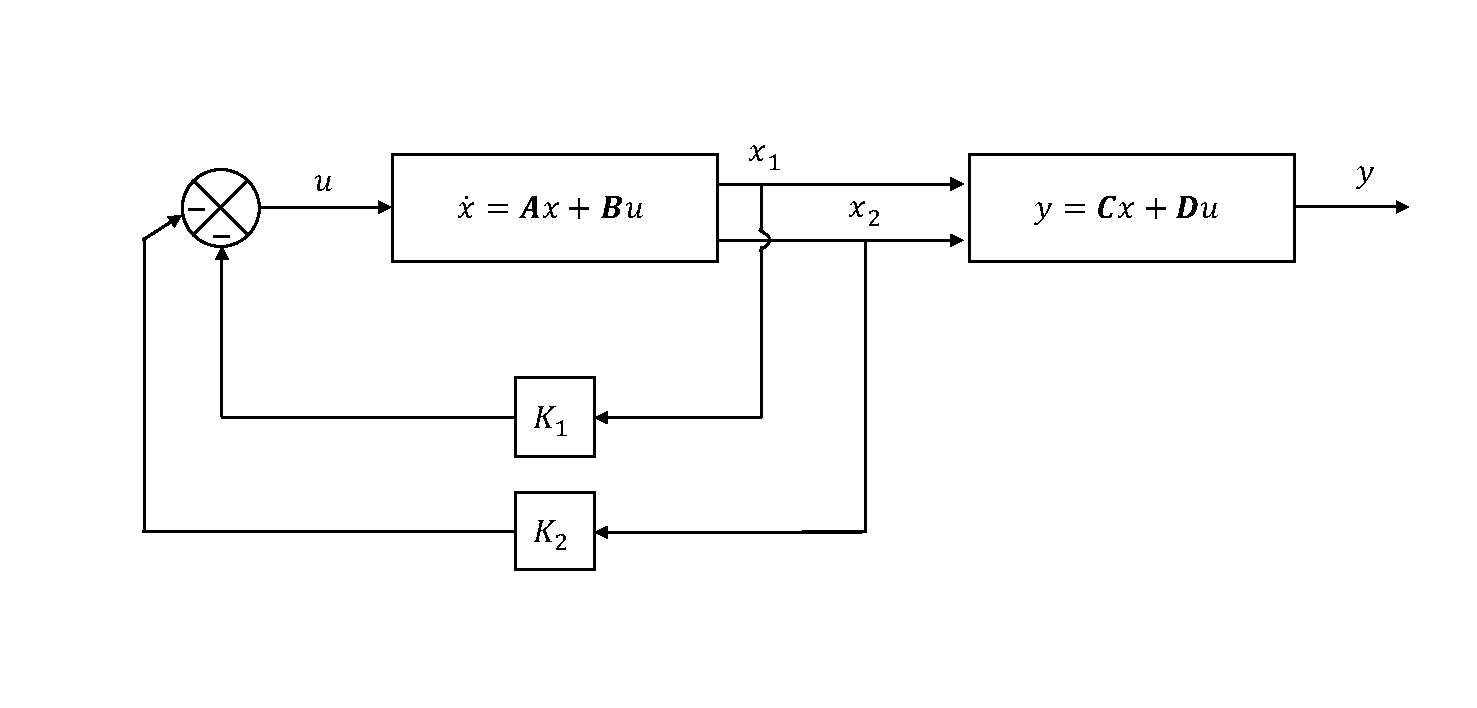
\includegraphics[scale=0.4]{diagrama.pdf}
\caption{Block diagram}
\label{fig:block_diagram}
\end{figure}

The state space representation \ref{eq:state_space}, \ref{eq:state_space_out} is a controllable canonical form that is important for the LQR controller design. It is desired to keep the actual ZMP, measured and computed by force-torque sensors located in the feet of the humanoid robot, close to its stable reference position as was discussed in previous sections. As the system is a type 0 plant, it is necessary to insert an integrator in order to design a ZMP servo control system (type 1) and remove the steady state error. Therefore, we feed the output signal $y$ (which indicates the real ZMP) back to the input and an integrator in the feedforward path as is shown in Figure \ref{fig:diagrama_int}.

\begin{figure}[!hbt]
\centering
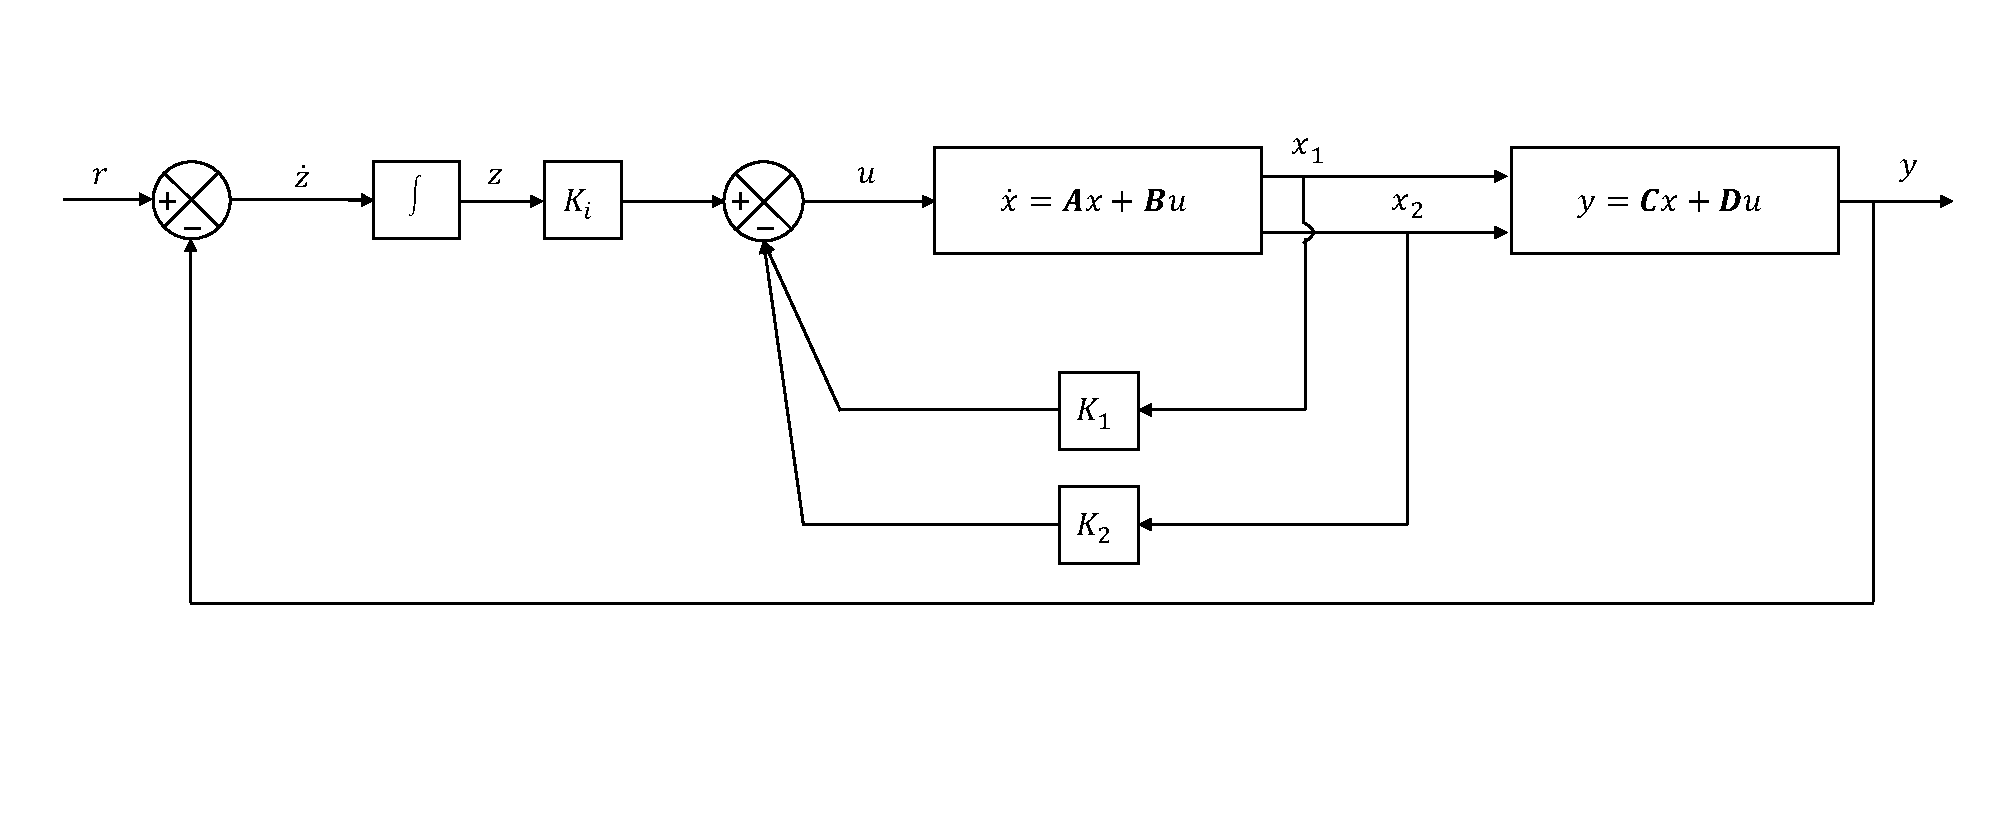
\includegraphics[scale=0.4]{diagrama_int.pdf}
\caption{ZMP LQR control system.}
\label{fig:diagrama_int}
\end{figure}

The optimum $K$ matrix is obtained from equations \ref{eq:Kcont} and \ref{eq:Kdisc}.
\begin{equation}
K = R^{-1}B^{T}P \quad (continuous \quad case)
\label{eq:Kcont}
\end{equation}
\begin{equation}
K = (R + B^{T}PB)^{-1}B^{T}PA \quad (discrete \quad case)
\label{eq:Kdisc}
\end{equation}

where $P$ is a positive-definite Hermitian or real symmetric matrix and it is necessary to compute the algebraic Ricatti Equation
\begin{equation}
P \rightarrow A^{T}P+PA-PBR^{-1}B^{T}P+Q = 0 \quad (continuous \quad case)
\end{equation}
\begin{equation}
P \rightarrow A^{T}PA+P-A^{T}PB(R+B^{T}PB)^{-1}B^{T}PA+Q = 0 \quad (discrete \quad case)
\end{equation}


In order to obtain the controller design for further simulations and experiments, the following mechanical parameters of the inverted pendulum (corresponding to Rh-2 humanoid robot) were taken: $m = 62.416 kg$, $l=0.8449 m$

\textcolor{red}{Valor de stiffness???}

For the optimum response of the control system, it is suggested to take $Q = C^{T}C = \begin{bmatrix}
5.037 \cdot 10^{-8} & 0\\
0 & 0
\end{bmatrix}$ and $R = 1 $. But for a faster response of the control, we take $Q = C^{T}C = \begin{bmatrix}
1000 & 0\\
0 & 0
\end{bmatrix}$.  After the LQR controller was designed, the control gains matrix $K = [23.1777 \quad 6.8027]$ was obtained.











